\section{Vision}

\subsection{Weather Rendering System}
This section defines a high-level vision for the desired outcome of this thesis and potential future work.
As listed in the primary goals, the weather rendering system will be based on compute shaders.
Compared to the prototype from the previous project, this is expected to result in a much better performance.
That in turn, allows for a more complex and realistic model.
\\
With the incorporation of real-time weather data and the use of topological landscape data, any given weather scenario could be simulated and rendered.
The desired outcome ideally looks similar to the image depicted in \autoref{img:rendered1}.
A rendered version of such a cloud system can look elusively realistic compared to an actual photograph, like in \autoref{img:photo1}.
\begin{figure}[ht]
    \centering
        \begin{minipage}{0.47\linewidth}
            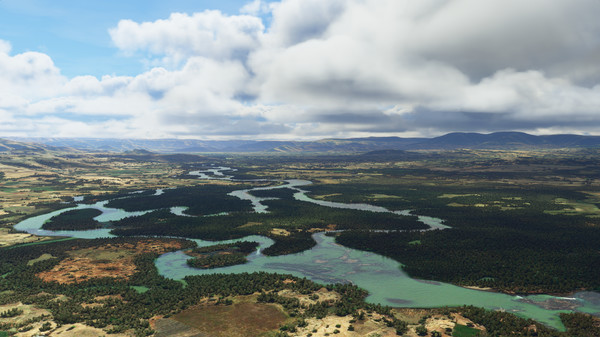
\includegraphics[width=\linewidth]{msfs-ref1.jpg}
            \captionof{figure}{A rendered image of volumetric clouds \protect\cite{img:rendered:clouds01}.}
            \label{img:rendered1}
        \end{minipage}
    \hfill
        \begin{minipage}{0.47\linewidth}
            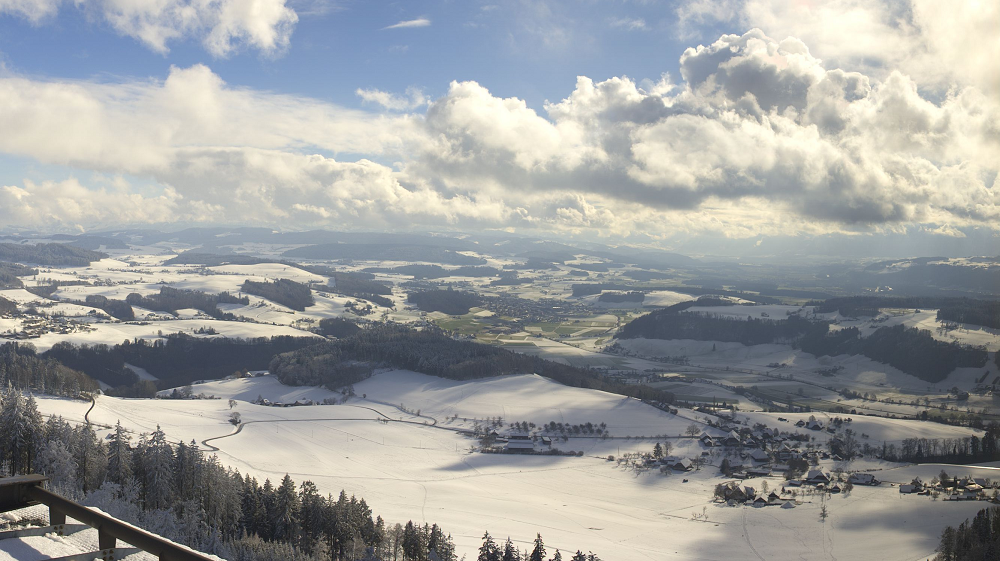
\includegraphics[width=\linewidth]{roundshot2021-01-18-12-50-cropped.png}
            \captionof{figure}{A photographic reference of clouds \protect\cite{img:photo:clouds01}.}
            \label{img:photo1}        
        \end{minipage}  
\end{figure}
\\
The first thought about the practical use of a fully-fledged volumetric cloud system might be a video game, since clouds are often a significant part of outdoor scenery in games.
However, for this thesis it is intended that the knowledge and results acquired during the given period will be used to recreate a lifelike weather system instead.

\clearpage

\subsection{System Overview}
To get a better understanding of how such a system could be implemented, this diagram shows all the involved components and their function.
\begin{figure}[H]
    \centering
    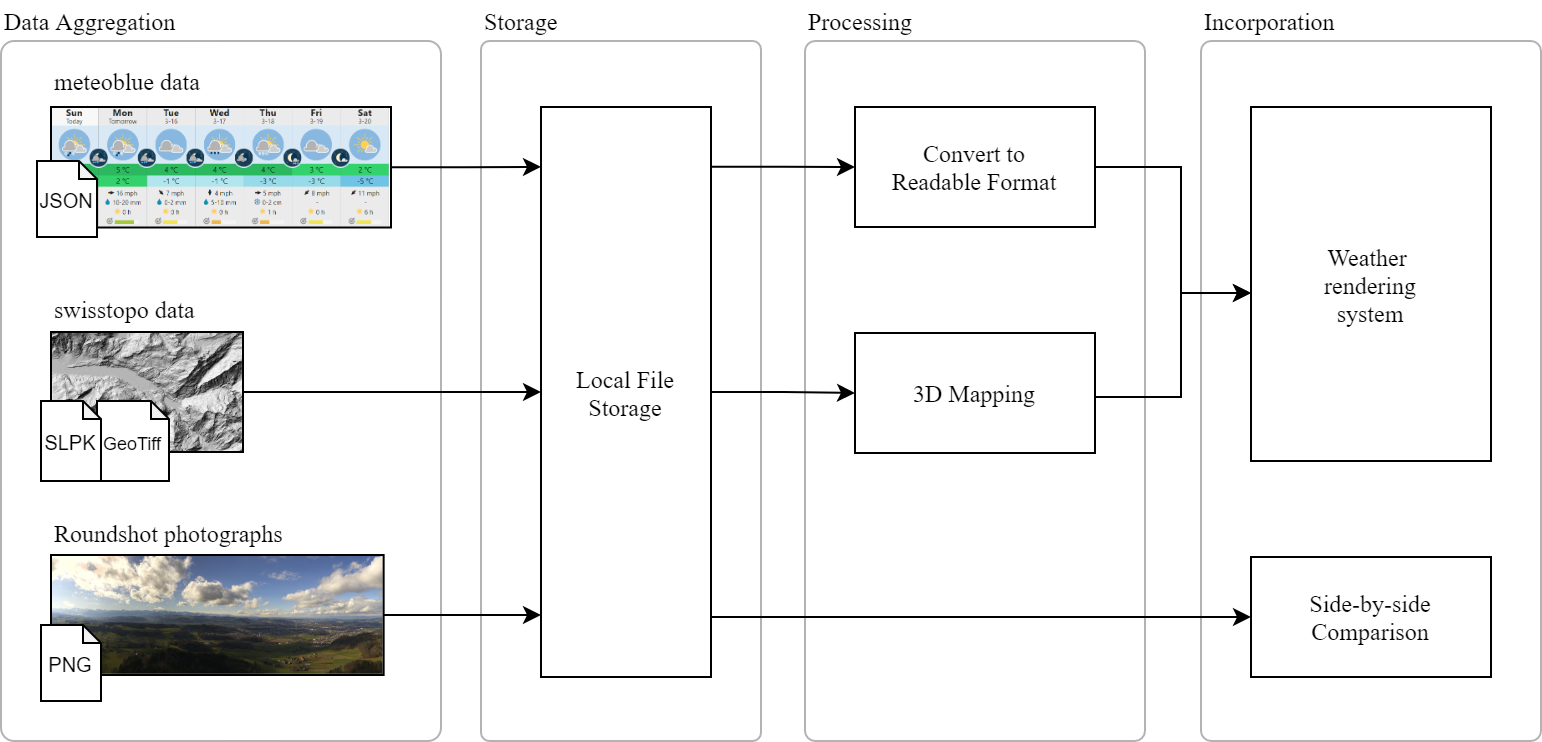
\includegraphics[width=\linewidth]{system diagram.png}
    \captionof{figure}{The system component diagram.}
    \label{img:systemoverview}
\end{figure}

\subsection{External Data}
\subsubsection{Meteoblue Weather Data}
To accurately reflect a weather system, conditions like precipitation, wind and cloudiness will be considered.
Fortunately, the company \emph{meteoblue} offers this data in form of different data packages \cite{meteoblue}.
As an additional bonus, the license costs are drastically reduced for student projects and educational work.
\\
From all available data packages, the "basic\textunderscore1h" \cite{meteoblue:basic1h} offer seems the most fitting for this thesis.
It includes the most common weather variables only, but this will clearly suffice for the planned project.
Some of the crucial variables are wind speed, wind direction, temperature, sea level pressure, and a pictocode.
\\
The weather data will be requested for the following locations:
\begin{itemize}
    \item Bern, Switzerland
    \item Fribourg, Switzerland \\(to account for the weather in the background of the photographs)
    \item Solothurn, Switzerland \\(to account for the weather in the background of the photographs)
\end{itemize}

\noindent
This data is retrieved on a daily basis and stored on a local file system for the duration of the thesis.

\subsubsection{Roundshot Photographs}
The weather data from \emph{meteoblue} gives detailed information about the weather at a specific time and date.
But to be able to compare the rendered result of the weather system with the actual weather of that period, real photographs of the same time should be used.
That is why images taken by the \emph{Roundshot} camera system from the company \emph{Seitz} \cite{roundshot} are stored periodically.
\\
There are many installations of those systems across the country. For this project, the following two locations are used: 
\begin{itemize}
    \item Roundshot camera Bantiger, Switzerland \cite{bantiger}
    \item Roundshot camera Gurtenpark, Switzerland \cite{gurtenpark}
\end{itemize}

\noindent
This data is retrieved on a weekly basis and stored on a local file system for the duration of the thesis.

\subsubsection{Swisstopo Height Models}
The last part of a convincing weather rendering system is the landscape. For that, the topologically accurate 3D height model data from the company \emph{swisstopo} will be used \cite{swisstopo}.
As of March 2021, \emph{swisstopo}'s height models and landscape data are available free of charge \cite{swisstopo:free}.
The goal is to download and convert this data into a Unity-compatible 3D model and use it as a base for the scenery.

\subsection{Future Work}
In a future project, the weather system could evolve into a complete flight simulation game where the player cruises through the clouds, like in Microsoft's \emph{Flight Simulator}.
Another interesting idea is to expand the system into a whole ecosystem with living creatures and animals. Their behaviour would be weather-dependent, making it one big symbiotic environment.